\section{Training}

\subsection{Training pipeline}

End-to-end document parsing requires both broad format learning and reliable structured generation. The model must convert a document page image into a Markdown representation while preserving text fidelity, formula renderability, table structure, reading order, and page-level completeness. These requirements call for supervision signals beyond token-level imitation, because many errors in tables, formulas, and long pages are easier to verify structurally than to express through next-token loss alone.

We therefore organize the training pipeline into stages with different roles. Supervised fine-tuning builds the initial end-to-end document parsing policy; reinforcement learning further improves the policy on hard pages using text, formula, and table rewards; on-policy distillation transfers the reward-aligned behavior of a 4B teacher into a deployable 0.8B student; model fusion then forms the final model.

\begin{figure}[!t]
\vspace{-0.3cm}
\centering
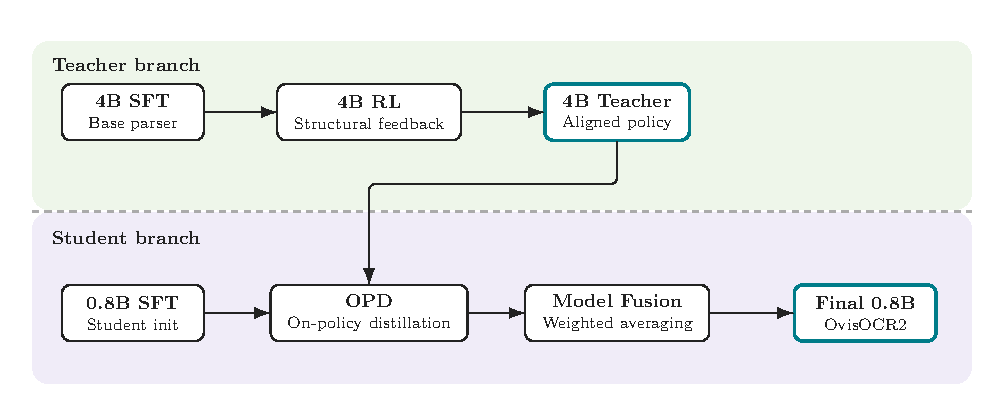
\includegraphics[width=\linewidth]{figures/training_pipeline.pdf}
\caption{Two-branch training of OvisOCR2. The 4B branch produces an RL-aligned teacher, while the 0.8B branch proceeds through SFT, OPD, and model fusion to obtain the final model.}
\end{figure}

\subsection{Supervised fine-tuning}

The SFT stage establishes the base policy for generating Markdown representations from document images. SFT uses the full data mixture described in the data section. The mixture is built on real document pages processed by the real-world data pipeline and is complemented by controlled samples from the synthetic data pipeline. Real data contribute natural layouts, scan quality variations, document types, and visual noise. Synthetic data increase the coverage of tables, formula-intensive pages, long Markdown outputs, and other long-tail structures. This stage therefore provides broad coverage and format consistency for the downstream RL and OPD stages.

We train both the Qwen3.5-0.8B and Qwen3.5-4B models with full-parameter SFT on the same document parsing objective. The 0.8B model is trained for two epochs, whereas the 4B model is trained for 20\% of an epoch to reduce the training cost of the larger branch. The 0.8B SFT checkpoint initializes the deployable student branch, while the 4B SFT checkpoint serves as the base policy for 4B RL; the resulting 4B RL checkpoint is then used as the OPD teacher. We use a 16K maximum sequence length together with a dynamic image-resolution budget, preserving fine-grained visual information without forcing all pages into a fixed resolution.

\subsection{Reinforcement learning}

RL further improves the end-to-end document parsing policy using reward signals on sampled outputs. Many important parsing errors are structural rather than purely lexical: a table may contain mostly correct text while having an incorrect cell topology; a formula may look similar as a string but fail to render or represent a different expression; long pages may suffer from omissions, repetition, or truncation. These errors are weakly expressed by token-level imitation loss, but they can be measured through programmatic checks, rendering-based comparison, and structure-aware parsing.

We use Group Relative Policy Optimization (GRPO)~\cite{shao2024deepseekmath} as the main RL algorithm. For each prompt, we sample multiple responses from the policy and compute group-relative advantages from verifiable rewards, without training an additional value model. This formulation is well suited to document parsing, where responses are long, structured, and evaluable by text, formula, and table analyzers. GRPO trains the model to prefer better candidates among multiple outputs for the same page, thereby reinforcing generation behaviors that are more complete, stable, and structurally valid.

\subsubsection{On-policy hard case construction}

RL data are constructed differently from the broad SFT mixture. The stage primarily uses samples from the synthetic data pipeline, where ground-truth structures are accurate enough to support text, formula, and table rewards. A smaller set of high-quality real documents is retained to preserve natural page distributions and varied visual conditions.

The training set is further shaped through on-policy filtering: we first run the current policy on candidate pages and score the generated responses with the reward function. Very easy and extremely hard samples provide little useful learning signal, and reward-flat samples with little variation across responses are less useful for group-relative learning. Training therefore emphasizes pages on which the model can occasionally produce responses that are clearly better than its average behavior.

\subsubsection{Multi-component reward design}

The RL reward is designed for complete page outputs and avoids reducing document parsing quality to a single text-similarity score. The scalar reward is computed from the components that are actually present in the ground truth: text, tables, and display formulas. Global validity checks, such as max-length truncation and unparseable structures, are applied as guards that zero out the affected available components rather than forming an independent reward term.

Table~\ref{tab:rl_feedback} summarizes the component scores used before page-level aggregation. CDM denotes character detection matching, an image-level metric for formula parsing~\cite{cdm}, and TEDS denotes a tree-edit-distance-based table similarity metric~\cite{pubtabnet}. In the reward, CDM and TEDS are used as normalized scores in \([0,1]\).

\begin{table}[!htbp]
\centering
\small
\setlength{\tabcolsep}{5pt}
\renewcommand{\arraystretch}{1.12}
\caption{Reward components used in RL.}
\label{tab:rl_feedback}
\begin{tabularx}{0.96\linewidth}{@{}>{\raggedright\arraybackslash\bfseries}p{0.22\linewidth}>{\raggedright\arraybackslash}p{0.28\linewidth}Y@{}}
\toprule
\textbf{Component} & \textbf{Score} & \textbf{Measured aspect} \\
\midrule
Text & 1 - normalized edit distance & Text fidelity \\
\addlinespace[2pt]
Formula & CDM & Visual formula matching \\
\addlinespace[2pt]
Table & TEDS & Table content and topology \\
\bottomrule
\end{tabularx}
\end{table}

Let \(\mathcal{C}=\{\mathrm{text},\mathrm{table},\mathrm{formula}\}\). For a page with prediction \(y\) and reference \(y^\ast\), \(s_c(y,y^\ast)\in[0,1]\) denotes the page-level score for component type \(c\). The text score is computed after page-level matching, while formula and table scores are averaged over evaluable ground-truth units after element matching and normalization. Each component has an availability indicator \(a_c(y^\ast)\), which equals one only when the reference contains at least one evaluable unit of that type. The page reward is then computed by averaging only the components available in the reference:

\[
R(y,y^\ast)
=
\frac{
\sum_{c\in\mathcal{C}} a_c(y^\ast)\,s_c(y,y^\ast)
}{
\sum_{c\in\mathcal{C}} a_c(y^\ast)
}.
\]

\subsubsection{Scalable multimodal RL training}

Multimodal RL training for document parsing needs to handle long text responses, page-level image inputs, and rendering-based reward computation. To make the training infra scalable, we apply the following optimizations.

First, reward computation uses hierarchical parallelism and shortcut paths. After rollout, page samples are scored by multiple reward workers in parallel. Within each worker, the formula reward performs matching and normalization first: normalized exact matches are assigned full credit directly, missing or invalid predictions are assigned zero, and only the remaining cases enter CDM rendering comparison. CDM computation is executed through a reusable process pool with per-task timeouts, preventing a small number of problematic formulas from blocking the worker. The table reward follows the same principle: normalized exact matches bypass TEDS, while invalid or unparseable tables receive zero. For long pages or abnormal outputs, the page-level matcher also uses timeout fallback to prevent matching from becoming a tail-latency bottleneck. Reward profiling is kept in the training loop so that slowdowns can be attributed to matching, normalization, rendering-based formula rewards, or table-structure scoring.

Second, the multimodal input transfer path is optimized for high-resolution document pages. Visual preprocessing can produce large page-level tensors, and repeatedly transmitting them across workers would increase host-side memory pressure and communication volume. Training therefore uses object-store-backed reference passing: large visual tensors are stored once and referenced by lightweight handles together with compact metadata. The policy update and reference-constraint computation retrieve and assemble the actual visual inputs when needed. This reduces transfer overhead and prevents high-resolution pages or long batches from moving the training bottleneck to serialization and data movement.

Third, the actor update is optimized for long responses. We use a common-prefix mask so that long shared prefixes among multiple rollouts of the same prompt do not dominate the loss, focusing gradients on tokens after the generation branches diverge. Under the strictly on-policy, single-epoch update setting, the system also avoids an additional old-policy probability pass. These optimizations reduce actor-side computation and memory pressure on long page outputs.

\subsection{On-policy distillation}

\subsubsection{Teacher-guided policy transfer}

A central challenge is to transfer the reward-aligned parsing behavior learned by the 4B RL model into a compact 0.8B model suitable for deployment. The 4B branch has greater capacity and can absorb reward signals more stably, while the compact branch is more sensitive to high-variance updates on long structured outputs. In our preliminary direct-RL comparison, applying the same RL stage directly to the compact model showed larger KL drift and less stable table quality, especially on dense pages and complex layouts.

\begin{figure}[!htbp]
\centering
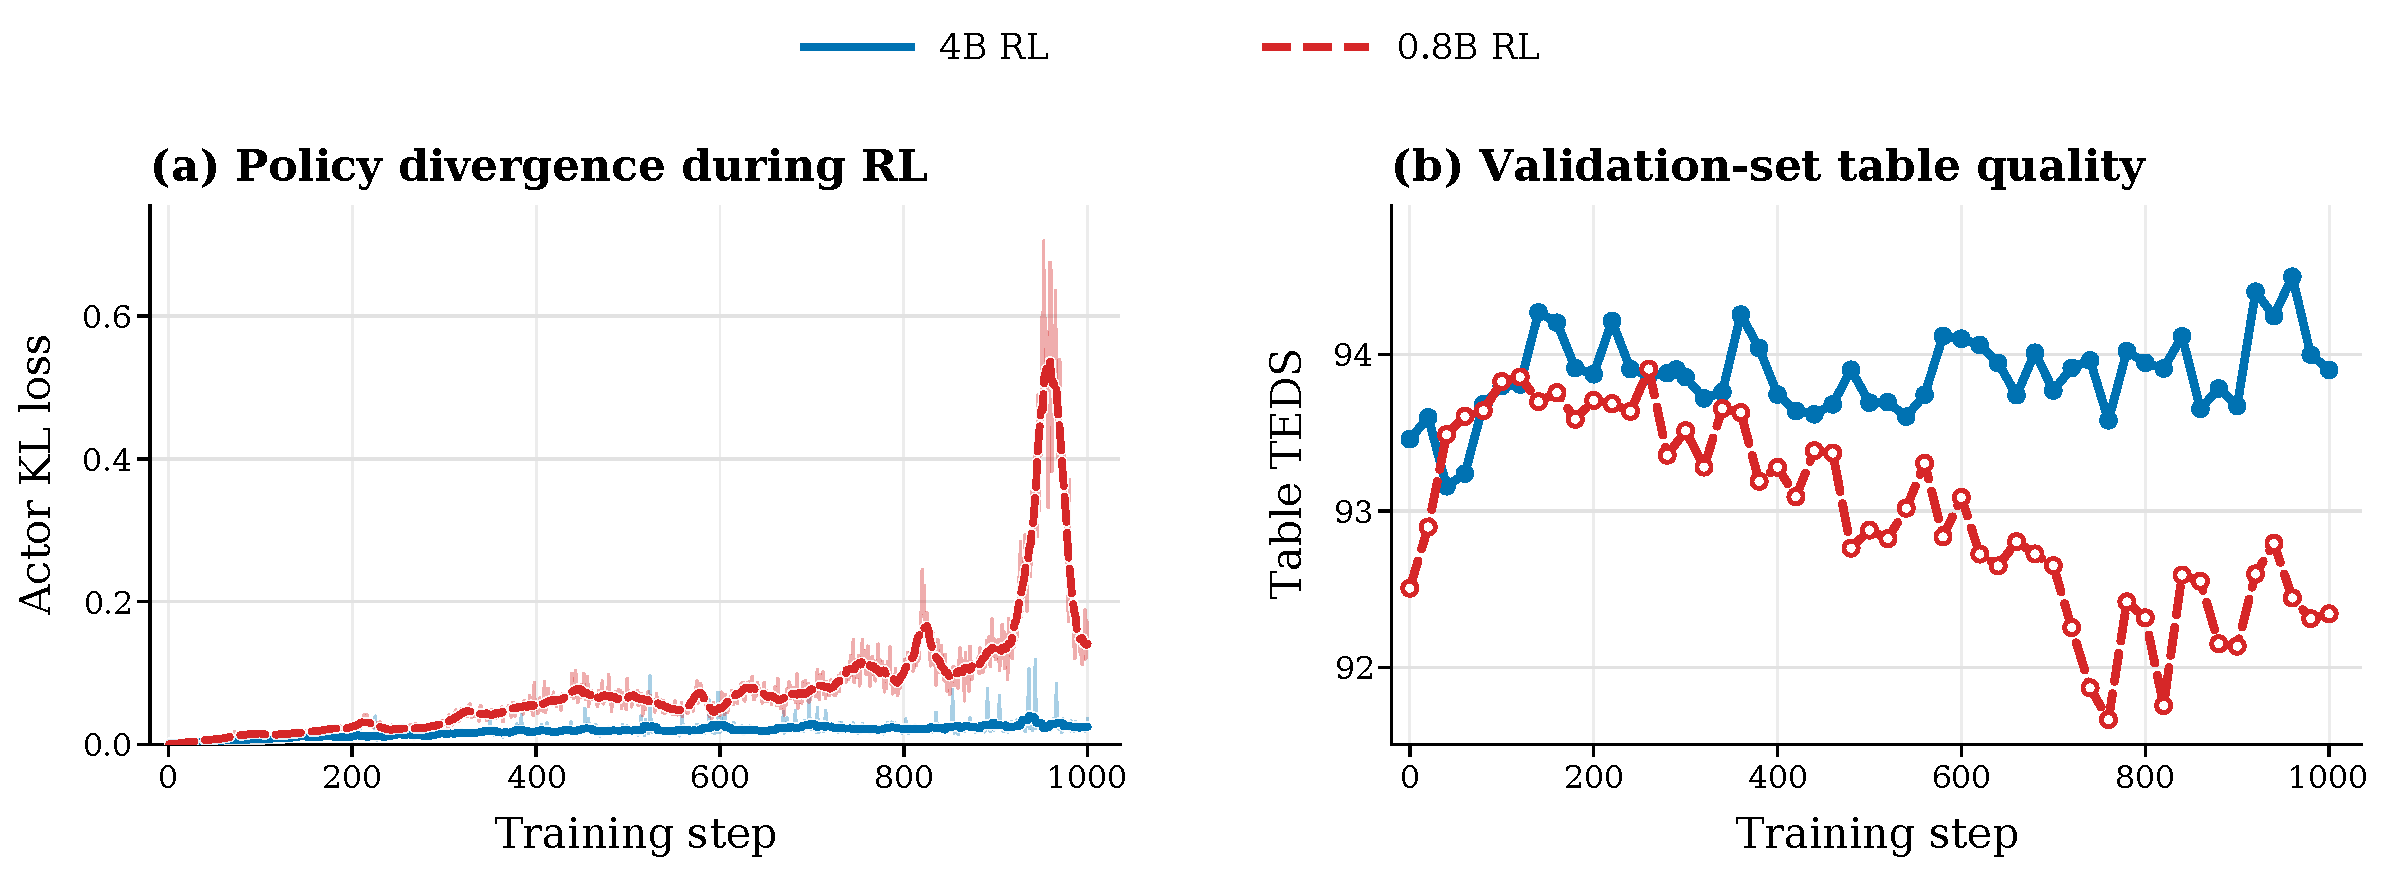
\includegraphics[width=\linewidth]{figures/rl_stability.pdf}
\caption{Training stability comparison between 4B RL and 0.8B RL. Panel (a) reports actor KL loss, with faint traces showing raw per-step values and bold curves showing 15-step centered rolling means. Panel (b) reports table TEDS on the validation set.}
\label{fig:opd_motivation}
\end{figure}

As shown in Figure~\ref{fig:opd_motivation}, direct 0.8B RL shows higher policy divergence in later training and a corresponding decrease in table quality compared with the 4B RL model. We therefore use the RL-enhanced 4B model as the teacher for the 0.8B student.

The student generates complete page outputs under its current policy, and the teacher evaluates these on-policy trajectories with token-level distribution supervision~\cite{hinton2015distilling,agarwal2024onpolicy}. The compact model thus receives the teacher's parsing preferences for tables, long formulas, and dense layouts through distribution matching, reducing the need to expose the student to another high-variance RL stage.

Formally, given a document image and instruction \(x\), the student policy \(\pi_\theta\) first samples a complete response \(y=(y_1,\ldots,y_T)\). The teacher policy \(\pi_\phi\) then evaluates conditional probabilities for candidate tokens under the same concatenated prompt-response context. Since the teacher and student share the same prefix \(c_t=(x,y_{<t})\), the loss does not require length alignment between teacher and student outputs; supervision is applied directly on states visited by the current student policy.

The main objective is student top-k reverse KL~\cite{li2026rethinkingopd}. At each response position, the support is determined by the current student distribution: \(S_t = \operatorname{TopK}_k\!\left(\pi_\theta(\cdot \mid c_t)\right)\). The teacher only needs to return log probabilities for tokens in \(S_t\). The student and teacher distributions are normalized within this support:

\[
\bar{p}_{t,v}
= \frac{\pi_\theta(v \mid c_t)}{\sum_{u \in S_t}\pi_\theta(u \mid c_t)},
\qquad
\bar{q}_{t,v}
= \frac{\pi_\phi(v \mid c_t)}{\sum_{u \in S_t}\pi_\phi(u \mid c_t)},
\qquad v\in S_t.
\]

Denote the resulting distributions over \(S_t\) by \(\bar{p}_t=(\bar{p}_{t,v})_{v\in S_t}\) and \(\bar{q}_t=(\bar{q}_{t,v})_{v\in S_t}\). Over the set of valid response token positions \(I\), the OPD loss is:

\[
L_{\mathrm{OPD}}(\theta)
=
\frac{1}{|I|}
\sum_{t \in I}
D_{\mathrm{KL}}\!\left(
\bar{p}_t \,\|\, \bar{q}_t
\right).
\]

Here \(I\) denotes token positions used for distillation, excluding prompt and padding tokens. The reverse-KL direction \(D_{\mathrm{KL}}(\bar{p}_t \,\|\, \bar{q}_t)\) gives the objective a mode-seeking behavior: within the compared support, it discourages student probability mass on tokens assigned low probability by the teacher, rather than pushing the student to spread probability over the teacher distribution.

\subsubsection{Efficient OPD training}

Full-vocabulary distillation is expensive for document parsing because page-level responses are long. For a response of length \(T\) and vocabulary size \(V\), matching teacher and student distributions at every response position would require \(T \times V\) log-probability tensors. By restricting the alignment to the student top-\(k\) support \(S_t\), the dominant tensor size is reduced from \(O(TV)\) to \(O(Tk)\).

Teacher scoring is performed on the student-generated trajectory. After student rollout, we keep the top-\(k\) token IDs at each response position and query the teacher for their log probabilities under the same prompt-response prefix. The student update uses the same token IDs. During the student forward pass, only the selected logits required by the OPD loss are gathered, and chunked projection is used for long responses to reduce peak memory.

\subsection{Model fusion}

We train several candidate \ours{} variants by varying both the data mixture and the training configurations. We then apply weighted parameter averaging~\cite{wortsman2022model} for model fusion, producing the final \ours{} model.
